\pagenumbering{arabic}

\chapter{Introduction}

\ifpdf
    \graphicspath{{introduction/figs/Raster/}{introduction/figs/PDF/}{introduction/figs/}}
\else
    \graphicspath{{introduction/figs/Vector/}{introduction/figs/}}
\fi


%\section[Short title]{Reasonably long section title}
Only a year after its invention in 1608, the optical device known as the telescope was first pointed to the sky \citep{histTel}. In the four hundred years since, the tool has not only been the driver of astronomical research but epitomises the field and its achievements. Aided by the finite speed of light, our place in the Universe is contextualised through glimpses into the past, revealing galaxies up to eight billion years old in the visible spectrum. As we approach the limits of optical telescopes, novel methods of astrophysical observation are needed for continued advancements in our understanding of the cosmos. One such method is the employment of an instrument used to study information encapsulated in electromagnetic waves beyond the visible regime; the radio telescope \citep{smithObsAst}.

Over the past century, astronomers have pieced together the chronology of the Universe with studies such as the JWST Advanced Deep Extragalactic Survey which has unveiled galaxies nearly 13 billion years old \citep{jades}. Continued measurements reveal more information and even older structures using data at longer wavelengths such as the infrared \citep{abyss} as the wavelength of light from the oldest structures stretches with the expansion of the universe. This phenomenon is known as ‘redshift’ and relates the wavelength of an observed signal to its original wavelength when emitted in the distant past
\begin{equation}
    \label{eqn:redshift}
    1 + z = \frac{ \lambda_{\mathrm{obsv}} }{ \lambda_{\mathrm{emit}} },
\end{equation}
where $z$ is the dimensionless redshift quantity while $\lambda_{\mathrm{obsv}}$ and $\lambda_{\mathrm{emit}}$ represent the signal's wavelength at the time of observation and creation respectively. Redshift can be related to the extent of universal expansion to show the ages of objects in the sky and it can be shown that information from the earliest stars and galaxies have redshifted out the regime of visible light and into lower wavelengths. Thus, probing the deepest cosmic questions such as the development of galaxies within the first billion years of our Universe requires the use of low-frequency techniques \cite{furPhys}.

Since the 1930’s, radio telescopes have remained one of the most exciting research areas in contemporary astronomy with their potential to explore the first hundreds of millions of years after the Big Bang through observation of redshifted signals. By the 1950’s it was understood that, being the most abundant material in the Universe, study of hydrogen and its interaction with astrophysical phenomena would trace the bulk evolution of the cosmos as a whole, especially during periods where there is no visible light to be seen such as before the first stars. While the ultimate goal of current experimentation would be to analyse images of primordial hydrogen \citep{liuData,21in21}, the limitations of current technology restrict us to an interim objective of spectral measurements from the early universe. An essential tool for astronomers hoping to examine this time period would be to take advantage of hydrogen’s preference for specific wavelengths of light (particularly those with a wavelength of 21 centimetres), which manifest as minute changes in temperature profiles where energy is absorbed or released by hydrogen.


% =========================================
\section{21-cm astrophysics}\label{sec:21cm}
Following recombination, remnant photons from the Big Bang pervaded the Universe having escaped the frenzied soup of electrons now confined into neutral hydrogen atoms held together in gaseous form \citep{ryden}. In the present day, the expansion of the Universe has stretched the wavelengths of these relic photons out of the visible spectrum and into microwave frequencies which have been measured as the cosmic microwave background (CMB)\footnote{In this text, the relic photon field and the CMB will be referred to interchangeably.}. These hydrogen atoms interact restrictively with the CMB via photons of wavelength equal to 21 centimetres \citep{lofar}. Hydrogen atoms absorb these 21-cm photons and gain their energy causing the orientation of ground state electrons to flip relative to their associated nuclei \citep{furProbe}. This marginally higher-energy hydrogen atom is said to be in an ‘excited’ state compared to its natural orientation. 

Initially, the transfer of electrons between the neutral hydrogen gas and the CMB was in equilibrium preserving the CMB spectra predicted by the Planck formula at radio frequencies. During this time, the orientation of electrons in hydrogen atoms, also referred to as the spin state, were continuously swapped in equal proportion. For every 21-cm photon absorbed by the CMB, another was emitted by some nearby hydrogen atom as it decays from an excited state. Soon afterwards but before the existence of the first stars, hydrogen atoms in dense pockets collide to temporarily form hydrogen molecules in a process known as collisional coupling \citep{21in21}. The combination of two atoms mixes the orientation of the constituent electrons which, through the Universe’s natural preference for low-energy states, leads to a net de-excitation of electrons when the pairs dissociate. This sweeping reset of electron orientations down to their lowest energy configuration breaks the equilibrium state as more de-excited hydrogen atoms are free to absorb 21-cm photons from the CMB. This loss of 21-cm photons by the CMB should be seen as minute deviations from the spectrum predicted by the Planck equation allowing us to timestamp the construction of dense hydrogen pockets that would eventually coalesce into the first stars. This collisional coupling is only temporary though, as the expansion of the universe cools hydrogen adiabatically returning the primordial gas to equilibrium with the CMB as shown in \cref{fig:reionisation_hist} \citep{21in21}. This collection of processes in the absence of luminous sources is referred to as the Dark Ages.
\begin{figure}
    \centering
    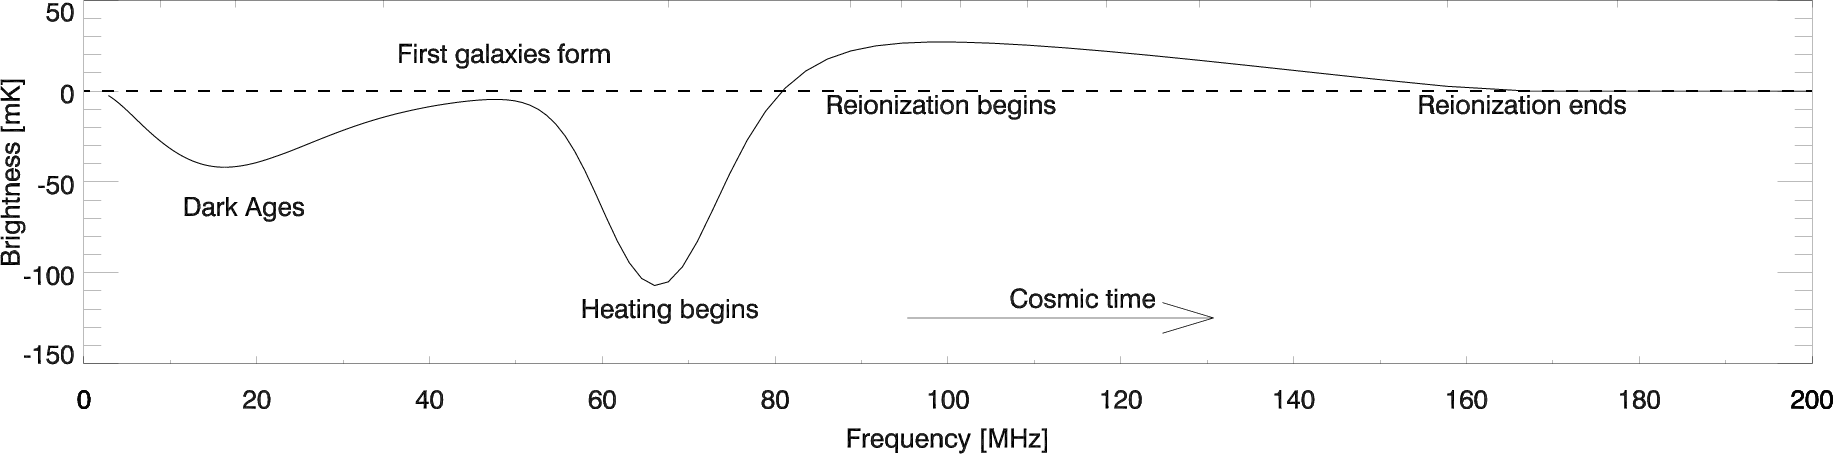
\includegraphics[width=\textwidth]{21cm_signal}
    \caption{A simulation of the expected 21-cm hydrogen signature based on typical models as a measurable brightness temperature (solid line) relative to the CMB temperature (dashed line). The turning points made from crests and troughs detail various stages of cosmic evolution such as the Dark Ages, the arrival of the first stars and galaxies, maturation of luminous sources and the Epoch of Reionisation. Image taken from \citet{cosmic_signature}.}
    \label{fig:reionisation_hist}
\end{figure}

The hydrogen gas in the most dense pockets eventually condenses into the first stars during Cosmic Dawn where ultraviolet (UV) radiation is generated for the first time since the Big Bang. Within this band of UV radiation are photons with a frequency of 2470 GHz known as a Lyman-$\alpha$ photon. These Lyman-$\alpha$ photons will bring the neutral hydrogen atoms to an energetic state beyond the spin flip which promptly decay down to the de-excited ground state, effectively cooling the gas and allowing for more absorption of CMB photons. This process, called the Wouthuysen-Field Effect, should yield an even stronger absorption trough than the collisional coupling as seen in \cref{fig:reionisation_hist} \citep{wouthuysen,field}. This first generation of stars will eventually mature into the first black holes and neutron stars producing even stronger radiation such as X-rays and gamma rays which will saturate the hydrogen gas and ionise them during an Epoch of Reionisation \citep{liuData}. The inability of hydrogen gas to continue absorbing photons will heat the gas past the CMB temperature leading to an emission profile as seen in \cref{fig:reionisation_hist}.

It is evident that CMB absorption and emission by primordial hydrogen gas traces early astrophysical processes that remain unconstrained by observation. Theory suggests that this may be measured as a differential brightness temperature relative to the predicted CMB profile and redshifted to radio frequencies between 50 and 200 MHz which can be represented by the equation
\begin{equation}
    \label{diffBright}
    \T{21} (z) \approx 0.023 \mathrm{K} \times x_{ \mathrm{H}_{\mathrm{I}} }(z) \left[ \left( \frac{0.15}{ \Omega_{\mathrm{m}} } \right) \left( \frac{ 1+z }{10} \right) \right]^{ \half } \left( \frac{ \Omega_{ \mathrm{b}} h}{0.02} \right) \left[ 1 - \frac{ \T{R}(z) }{ \T{S}(z) } \right],
\end{equation}
and is dependent on many characteristics of the early universe such as the fraction of hydrogen gas that is neutral $x_{ \mathrm{H}_{\mathrm{I}} }(z)$, the matter and baryon densities with respect to the critical density of the Universe $\Omega_\mathrm{m}$ and $\Omega_\mathrm{b}$ as well as Hubble’s constant $h$ \citep{edgesNature}. Also present in the equation is the temperature of the background radiation $\T{R}$ and the spin temperature $\T{S}$ which represents the relative populations of excited and de-excited electrons\footnote{The factor of 0.023 K comes from atomic-line physics \citep{edgesNature}}. Qualities of early luminous sources such as the efficiency of star formation or the mean free path of ionising photons will affect heating and alter the profile of the differential brightness temperature, producing a unique 21-cm brightness temperature such as the models shown in \cref{fig:21cm_models} where each individual line corresponds to a possible cosmic history \citep{theory_models}. Working backwards from an observed signal would provide constraints to these parameters narrating the influence of the first structures on the primordial hydrogen.
\begin{figure}
    \centering
    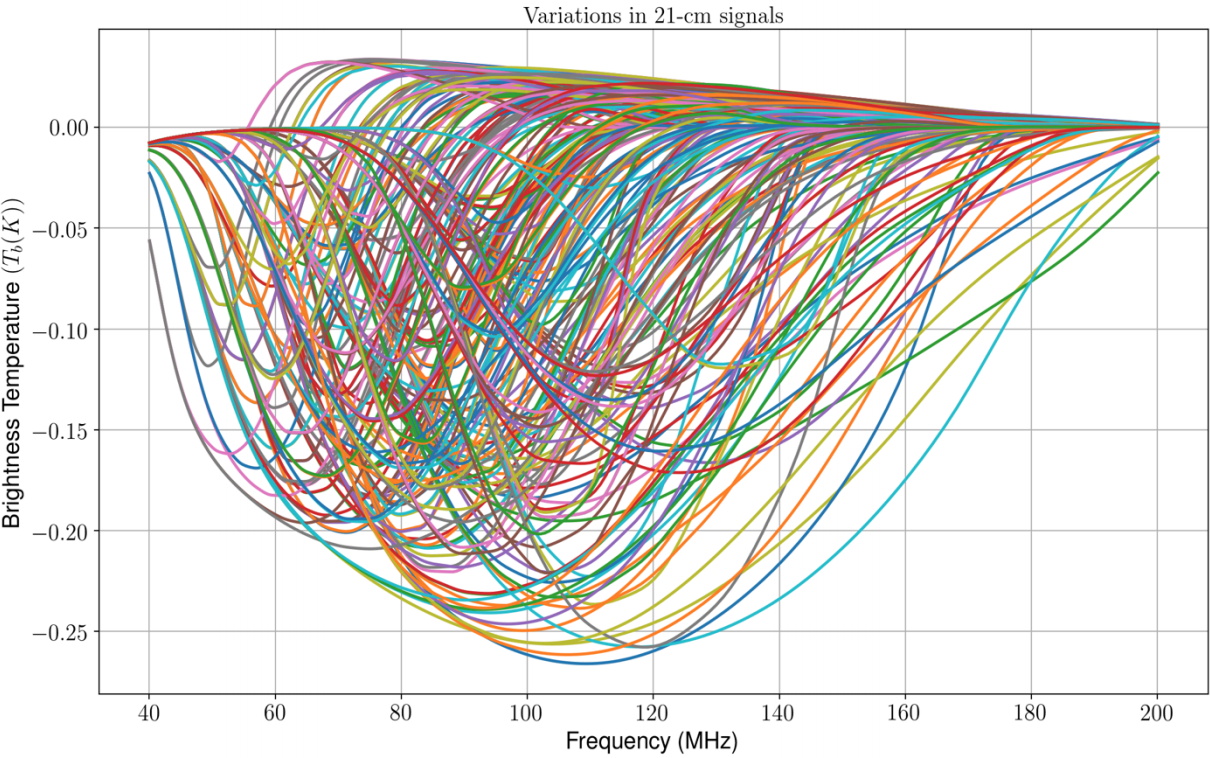
\includegraphics[width=0.8\textwidth]{21cm_models}
    \caption{Numerous simulations of plausible hydrogen signatures each representing a possible cosmic history. Various parameters such as the precise arrival of the first stars and galaxies will alter the hydrogen signal which when compared will allow theoreticians to identify models most representative of our early Universe. Data for image taken from \citet{theory_models}.}
    \label{fig:21cm_models}
\end{figure}


With the potential to provide such a wealth of information, many experiments have attempted to measure the 21-cm signature by taking long time integrations of radio spectra as a function of frequency averaged over the entire sky, also known as a ‘global’ measurement. This method has been employed in projects such as the Broadband Instrument for Global Hydrogen Reionisation Signal (BIGHORNS) \citep{bighorns}, the Large-Aperture Experiment to Detect the Dark Ages (LEDA) \citep{leda}, the Shaped Antenna Measurement of the Background Radio Spectrum (SARAS) \citep{saras} and the Sonda Cosmol\'{o}gica de las Islas para la Detecci\'{o}n de Hidr\'{o}geno Neutro (SCI-HI) \citep{scihi}. Another method of observation is the utilisation of interferometric arrays to measure spatial fluctuations in the sky brightness temperatures on the scales of megaparsecs which would give details on individual luminous sources. This technique is used in experiments such as the Low-Frequency Array (LOFAR) \citep{lofar}, the Precision Array for Probing the Epoch of Reionization (PAPER) \citep{paper}, the Hydrogen Epoch of Reionization Array (HERA) \citep{hera} as well as the future Square Kilometre Array (SKA) \citep{ska}.

Despite the developments in radio astronomy, a definitive detection of the 21-cm signature is yet to be made due to the difficulties that arise from such a measurement. One hindrance to experimentation are astrophysical foregrounds that may be up to five orders of magnitude higher than the proposed hydrogen signal at radio frequencies. These foregrounds include radiation produced from cosmic ray electrons moving through magnetic fields in our galaxy known as galactic synchrotron radiation, or the emission of photons when electrons scatter of the presently-ionised hydrogen nuclei known as free-free emission \citep{foregrounds,edges}. Fortunately, it is thought that the various crests and troughs of the 21-cm signature, known as ‘turning points’, allow the hydrogen signal to be distinguishable from the foregrounds which are smooth at radio frequencies and approximated by simple power law equations \citep{edgesNature}. Another point of concern are TV and FM radio broadcasts which are emitted at the frequencies relevant to 21-cm experiments \citep{reach}. Earth’s atmosphere is also known to be refractive at radio frequencies causing any potential signal to wander around the sky as ionospheric patches roll past the telescope’s observational beam \citep{lofar}. In response to these challenges however, scientists have developed models and methods to mitigate the effects of such impedances enabling continued studies which have provided intriguing results.


% =========================================
\section{The EDGES experiment}\label{sec:edges}
To date, the most significant result in 21-cm experimentation has been made by the Experiment to Detect the Global EoR Signature (EDGES) which aims to detect the sky-averaged 21-cm brightness temperature from the EoR \citep{edgesCal}. The project has been conducting multiple observations from the Murchison Radio-astronomy Observatory in Western Australia since 2006 \citep{edgesCal} using multiple dipole-like antennas of metal panels mounted horizontally above a ground plane \citep{edgesNature}. Early measurements placed an upper limit on the relative brightness temperature of the redshifted 21-cm signal contribution to their recorded foreground-removed spectrum \citep{edges2008} as well as a lower limit to the duration of the reionisation epoch with $\delta z > 0.06$, the latter result effectively excluding rapid reionisation models \citep{edges2010}. Following the deployment of one high-band and two low-band instruments, EDGES reported the detection of a flattened absorption profile in the radio spectrum centred at 78 MHz with a width of 19 MHz and depth of 0.5 K which they suggest is the 21-cm hydrogen signature \citep{edgesNature}.

The finding was met with considerable discussion as the detected profile’s characteristics did not match theoretical models. The trough centering at 78 MHz (corresponding to a redshift $z \sim 18$) would require more efficient star and galaxy formation at high redshifts \citep{edges_star_formation} while its flattened Gaussian shape suggest a delayed start to X-ray heating after the formation of Lyman-alpha emitting stars, not consistent with models \citep{theory_models}. Most notably however, was the profile amplitude which is more than a factor of two greater than the largest predictions by \citet{theory_models} as shown in \cref{fig:edges_signal} which would indicate that either primordial gas was cooler than expected or that the background radiation temperature was hotter than expected \citep{edgesNature}. With both the radiation and gas temperatures constrained by the CMB and adiabatic cooling mechanisms, known astrophysical processes are unlikely to account for the observed discrepancy and new physics has been proposed to to rectify the inconsistency such as an IGM cooling channel facilitated by dark matter-baryon interactions \citep{edgesNature}. Other phenomena such as an excess radio background due to efficient black hole formation obscured by dense hydrogen halos have also been proposed \citep{ew_radio_background}.
\begin{figure}
    \centering
    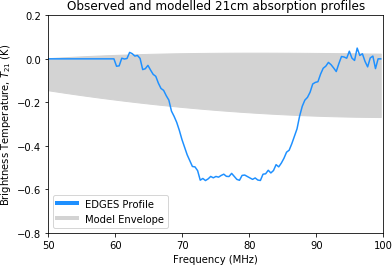
\includegraphics[width=0.7\textwidth]{edges_signal}
    \caption{The detected EDGES profile shown in blue \citep{edgesNature} over an envelope of models from \cref{fig:21cm_models} shown in grey. It is evident that the EDGES signal exhibits and absorption trough that is is deeper than all of the models shown. If astrophysical, this suggests and increased amount of CMB photon absorption by neutral hydrogen gas than previously expected. Additionally the flatness and width of the absorption trough are also unlike the models shown in \cref{fig:21cm_models}. All of these differences which may require new physics to explain. Data for EDGES signal available in footnote link \textsuperscript{c}. Data for model envelope from image by \citet{theory_models}.}
    \label{fig:edges_signal}
\end{figure}

Alternatively, inaccurate analysis methods or instrumental systematics may also account for the disparity between the EDGES data and theoretical models. \citet{hills_concerns} showed that the EDGES modelling process implied unphysical foreground emission parameters while \citet{sims_concerns} describe systematic calibration errors preferred by the Bayesian evidence under statistical analyses of the publicly available EDGES data\footnote{available at \url{http://loco.lab.asu.edu/edges/edges-data-release/}}. The \mbox{SARAS 3} radiometer measuring radio sky spectra at 55--85 MHz tested for the presence of the EDGES best-fit profile which was rejected from their data at the 95.3\% confidence level \citep{saras_reject}. Furthermore upper limits on the 21-cm power spectrum set by HERA Phase I observations were found to neither support nor disfavour a cosmological origin to the feature seen by EDGES \citep{hera_limits}.


The divided interpretation of the profile centred at 78 MHz highlights the need for follow-up experimentation to definitively confirm or refute the findings of \citet{edgesNature}. Continued investigations will need to improve on the instrumentation, analysis methods and measurement techniques in order to avoid data of nebulous origin or questionable interpretation. Many projects such as Probing Radio Intensity at high-Z from Marion (PRIZM) \citep{prizm}, Mapper of the IGM Spin Temperature (MIST) \citep{mist} and the Dark Ages Polarimeter PathfindER (DAPPER) \citep{dapper} are spearheading the effort including a certain Cambridge-led collaboration…


% =========================================
\section{The REACH experiment}\label{sec:reach}
The Radio Experiment for the Analysis of Cosmic Hydrogen (REACH) is a Cambridge-led sky-averaged 21-cm experiment of which the author is a member of. The radiometer targeting the cosmic hydrogen signature between 50--170 MHz ($z \sim $7.5--28) has a principle science objective of verifying the EDGES detection through a phased deployment at the RFI-quiet Karoo South African radio reserve \citep{reach}. A design focus on the identification and removal of residual systematics sets REACH apart from concurrent experiments which typically aim to minimise the chromatic response of the instrument as achromatic antennas mitigate the introduction of spectral components into foreground signals \citep{edges2008,saras2}. Relying on such a ‘smooth’ instrument response presents challenges such as with EDGES where the resulting frequency bandwidth ratio is restricted to 2:1 necessitating the use of scaled systems with overlapping bands to cover the full frequency range. REACH alternatively intends to improve on current experiments through the joint detection and characterisation of instrument systematics together with astrophysical foregrounds and the cosmic signature using Bayesian statistical methods \citep{dom,dom_modelling}. This joint fit between physically-based models is expected to facilitate the detection of correlated systematics and avoid those potentially degenerate with a cosmological signal with unaccounted-for systematics diagnosed using Maximally Smooth Functions \citep{maxsmooth}.

REACH Phase I plans on taking simultaneous observations of the sky using two antennas; the hexagonal dipole (50--130 MHz) and the conical log spiral (50--170 MHz) both of which were chosen from numerous designs for their ability to reconstruct mock 21-cm signals to a high degree of statistical confidence with small root mean square error in simulations \citep{dom_antenna}\footnote{We note that the hexagonal dipole is similar to the rectangular dipole antenna used in the EDGES experiment}. The antenna pair will be analysed in parallel to isolate signal components associated with hardware systematics while the contrasting mechanical designs will prevent experimental sensitivity to hardware-specific systematics. The project’s non-reliance on achromatic antennas allows for an ultra-wideband system covering the Cosmic Dawn and EoR (up to 3.5:1 for the conical log spiral) \citep{john_antenna}. Using such a large bandwidth, spectral differences between the oscillating 21-cm signature and the smooth power-law foregrounds can be leveraged during data analysis to support a positive detection \citep{reach}.

The deployment site was also chosen with care after an extensive survey. In the Karoo, REACH will observe the southern hemisphere sky from a remote 4 km wide basin surrounded by hills and mesas offering a reduced FM radio presence. Located near similar experiments such as HERA, MeerKAT \citep{meerkat} and the Square Kilometre Array (SKA)1-Mid instrument \citep{ska}, the location offers critical support infrastructure including on-site maintenance, staff as well as controlled access through paved roads. A Phase II experiment is planned for the same site which will incorporate additional antenna systems. Scaled versions of the hexagonal dipole and dual polarisation antennas have been proposed.

Simulations run with the above specifications forecast percent-level constraints on astrophysical parameters using REACH and in the case of a non-detection, upper limits on the strength of the absorption feature can be used to bound high-redshift phenomena \citep{reach}. We estimate a $\sim 500$ mK absorption profile consistent with EDGES can be detectable in as little as three hours of integrated data out of approximately 30 hours of observation time ($\lesssim \frac{1}{6}$th the time necessary to detect more conservative 21-cm signature models at the same redshift), though up to an order of magnitude more time may need to be allocated for the removal of low quality data and calibration measurements. If the data do not support an EDGES-like or high-amplitude 21-cm signal, the experiment will continue to integrate for longer periods in which case REACH will be able to place rigorous constraints on any excess radio background amplitudes and hydrogen cooling mechanisms beyond the typical adiabatic expansion. For the case of a detected 21-cm absorption signature much smaller than the EDGES profile in the high signal-to-noise regime, forward modelling consistent with standard astrophysics and cosmology will be used to constrain parameters such as the low-energy cutoff frequency and power law index of the X-ray spectral energy distribution, the X-ray efficiency of sources, the CMB Thomson-scattering optical depth, the minimum virial circular velocity of star-forming galaxies, the mean free path of ionising photons in the IGM as well as the star-formation efficiency \citep{tom_crh,visbal,fialkov_history}.

Contingent on this detection is of course, the measurement accuracy and sensitivity of the instrument as a whole. The contribution to this project by the author is the maximisation of such attributes through the construction of a high quality radio-frequency receiver unit, its seamless incorporation within the overarching system, as well as the development of intelligent software for receiver calibration. In this thesis, we present the designs, motivation, specifications and production of the REACH front-end and back-end receiver unit for deployment in 2023 highlighting its unique architecture and features to aid in instrument characterisation. We also detail an innovative calibration procedure that incorporates a Bayesian methodology leading to an in-field, rapid algorithm for calibration of the instrument in the same environment as observations, a first of its kind. While presenting the results of the technique, we highlight the challenges of achieving the accuracy needed to detect such miniscule 21-cm signals as well as present a framework for continued advancements in calibration towards the detection of the highly-redshifted global 21-cm hydrogen signature.

